\section{Adversarial Examples の実験方法と典型的なデータセットの解説}
\label{sec:exp-design-and-data}
この章では、adversarial examples の実験として用いられる典型的な手順を解説すると共に, 実験でよく使われるデータセットを解説する.



\subsection{Adversarial Examples の実験方法}
\label{subsec:exp-design}
adversarial examples を使った実験は大別すると以下の 3 つの目的から成る.
%
\begin{itemize}
  \item 攻撃目的\\
  モデルの正答率を下げるために adversarial examples を使う.
  攻撃はモデルの正答率を低くするほど、効率的(計算量が少ない、adversarial examples を作成するために必要なシステムへのクエリ回数が少ない、など)であるほど良い攻撃であると解釈される.
  モデルの正答率を表記する場合とモデルの誤認識率(1 - 正答率)を表記する場合がある.
  \item 防御目的\\
  モデル学習時に adversarial examples を使うことで, 攻撃に対して耐性を高める.
  防御はモデルの正答率を高めるほど良い防御であると解釈され, この観点だけを議論している研究が多い.
  実運用を考えれば防御方法は効率的(導入の人的・計算資源的コストが少ない、推論時の速度に対する影響が少ない、など)であるほど好ましいが, このような観点を議論している研究はまだあまり見かけない.
  \item データやモデルを理解する目的\\
  adversarial examples はモデルに対する特殊なバグのようなものでなくデータに内在する特徴である \cite{ilyas2019adversarial} と捉えたり, adversarial examples を使って overfitting を検出する \cite{werpachowski2019detecting} など, データやモデルの特徴を理解するために adversarial examples を使う.
  これらは adversarial examples の活用として興味深い方向性ではあるが, 本書では扱わない.
\end{itemize}
%

攻撃目的の実験はシンプルだが, 防御目的の実験は注意が必要である.
登場するデータを整理しながら典型的な防御目的の実験手順を見ていく.

データの集合としては元々の教師データの集合 $\mathcal{D}_{\text{clean}}$ があり, これは train/test を含んでいる.
少し冗長ではあるが, ここでの説明に限りそれらを $\mathcal{D}_{\text{clean, train}}, \mathcal{D}_{\text{clean, test}}$ と表記する.

防御方法で adversarial examples を使う場合には, train に対応する $\mathcal{D}_{\text{adv, train}}$ を作成し学習に利用する\footnote{
これを使わずに防御する手法も数多く提案されているため, 必ず使うわけではない
}.
テスト時には, 学習したモデルを攻撃するための $\mathcal{D}_{\text{adv, test}}$ を作成し, これに対する正答率を測ることで防御方法の性能を議論する.

この手順のみに注目している研究も少なくないが, 実際には防御方法を入れたことによって $\mathcal{D}_{\text{clean, test}}$ に対する影響が生じ得るため, このデータに対する正答率も合わせて評価するのがより正しい手順となる.

本書では画像データのみに着目するためこのような説明となっているが, 自然言語処理では学習時に adversarial examples を利用するのは防御のためというより $\mathcal{D}_{\text{clean, test}}$ に対する正答率を高めるためという目的で使われることが多い\footnote{
もちろん画像データでもそのような目的で adversarial examples を使っているものがあり, 例えば \cite{xie2019adversarial} などが挙げられる.
}.
このような背景もあり, adversarial examples を用いた学習で汎化性能を向上させる, というような言及がある場合は $\mathcal{D}_{\text{clean, test}}$ に対するものか $\mathcal{D}_{\text{adv, test}}$ に対するものかを文脈から判断する必要がある.
本書における防御方法の実験では, 必ず両方のデータで正答率を評価するようにしている.



\subsection{Adversarial Examples の実験でよく使われるデータセット}
\label{subsec:typical-dataset}
adversarial examples の実験でよく用いられるデータセットを紹介する.
部外者がアクセスできない論文独自のデータセットは取り上げず, オープンアクセスのデータセットのみを対象とする.

train/test の画像枚数, 画像サイズ [channel, height, width], クラス数, 簡単な特徴をデータセット毎に記載する.
%
\begin{itemize}
  \item MNIST \href{http://yann.lecun.com/exdb/mnist/}{http://yann.lecun.com/exdb/mnist/}\\
  train/test : 60,000/10,000\\
  画像サイズ : [1, 28, 28]\\
  クラス数 : 10\\
  特徴 : 手書き数字文字 (0 から 9 まで) のデータセット.
  \item fashion MNIST \href{https://github.com/zalandoresearch/fashion-mnist}{https://github.com/zalandoresearch/fashion-mnist}\\
  train/test : 60,000/10,000\\
  画像サイズ : [1, 28, 28]\\
  クラス数 : 10\\
  特徴 : MNIST のファッション画像版のデータセット. クラスは T シャツやズボンなど.
  \item CIFAR10 \href{https://www.cs.toronto.edu/~kriz/cifar.html}{https://www.cs.toronto.edu/~kriz/cifar.html}\\
  train/test : 50,000/10,000\\
  画像サイズ : [3, 32, 32]\\
  クラス数 : 10\\
  特徴 : 飛行機や車などの互いに overlap がない排他的なクラスのデータセット.
  \item CIFAR100 \href{https://www.cs.toronto.edu/~kriz/cifar.html}{https://www.cs.toronto.edu/~kriz/cifar.html}\\
  train/test : 50,000/10,000\\
  画像サイズ : [3, 32, 32]\\
  クラス数 : 100\\
  特徴 : CIFAR10 のクラス数を増やして 1 クラス毎の画像枚数を減らしたデータセット.
  \item SVHN \href{http://ufldl.stanford.edu/housenumbers}{http://ufldl.stanford.edu/housenumbers}\\
  train/test : 73,257/26,032 (追加学習用の 531,131 件のデータもある)\\
  画像サイズ : [3, 32, 32]\\
  クラス数 : 10\\
  特徴 : Google Street View Image から取得した数字画像のデータセット. 実験でよく使われるのは一枚の画像に一つの数字が写るように 32 * 32 に切り出した画像(実際には一枚の画像に複数の数字が写り込むものも多い)だが, 切り出す前の解像度がバラバラの元データも提供されている.
  \item GTSRB \href{https://www.sciencedirect.com/science/article/abs/pii/S0893608012000457?via\%3Dihub}{https://www.sciencedirect.com/science/article/abs/pii/S0893608012000457?via\%3Dihub}\\
  train/test : 39,209/12,630\\
  画像サイズ : カラー画像で height と width はバラバラで, それぞれ平均は 50 程度.\\
  クラス数 : 43\\
  特徴 : ドイツの標識のデータセット. 標識部分を切り出し, 標識の種類が分類クラスになっている.
  \item ILSVRC \href{http://www.image-net.org/challenges/LSVRC/}{http://www.image-net.org/challenges/LSVRC/}\\
  train/valid : 1,281,167/50,000 (\href{https://www.tensorflow.org/datasets/catalog/imagenet2012}{https://www.tensorflow.org/datasets/catalog/imagenet2012})\\
  画像サイズ : カラー画像で height と width はバラバラで, 平均は (450, 400) 程度.\\
  クラス数 : 1,000\\
  特徴 : 画像分析のコンペティションで用いられる大規模データセット. 年によってデータに変更が加えられるが, classification は 2012 から変わらないので ILSVRC2012 のデータと表記して使用することが多い. サイズは [3, 224, 224] や [3, 299, 299] で使うことが多い. ダウンロードするには \href{http://www.image-net.org/download-images}{http://www.image-net.org/download-images} で登録が必要.
\end{itemize}
%

adversarial examples に用いるデータとして道路標識を使う場合は少なくないが, それには以下のような理由が挙げられる.
%
\begin{itemize}
  \item 対象物としてシンプルなので摂動が認識しやすいため, どうやって認識しづらい摂動を作成するかという観点で興味深い
  \item 距離や角度や明るさといった物理的環境条件が頻繁に変更される状況で認識をしなければならないため, robust な摂動を構築するという観点で興味深い\footnote{
  robust という言葉はモデルの汎化性能を表現するために使われることが多いが, adversarial examples の文脈では距離や角度などが異なる環境条件で撮影した画像であっても同じように誤認識を引き起こすことができる摂動を robust と呼ぶことも多い.
  やや confusing な言葉の使い方ではあるが, 慣例に従い本書でも robust な摂動などと使うことにする.
  }
  \item 上の項目と近しいことだが, 現実的な攻撃は物理的環境条件が変化する状況で実施することが自然であり, 道路標識はそのような状況を作りやすいので実際に生じうる脅威として検討できる
  \item 画像認識の性能に強く依存していて, かつ誤認識が深刻な問題となりうる自動運転にとって重要
\end{itemize}
%
似たような対象としては人体検出なども挙げられるが, 本書では扱わない.

ここで挙げたデータセットの画像例を図 \ref{fig:typical-dataset-samples} に載せている.
解像度の低い画像で様々なラベルが存在する CIFAR は人間の目では何が写っているかよく分からないものも存在する.
adversarial examples の実験ではコストを抑えるために低解像度の画像を用いるものも多かったが, 評価としては不十分な面もあるため近年になって ILSVRC2012 が用いられることも増えてきている.
%
\begin{figure}[htbp]
\begin{center}
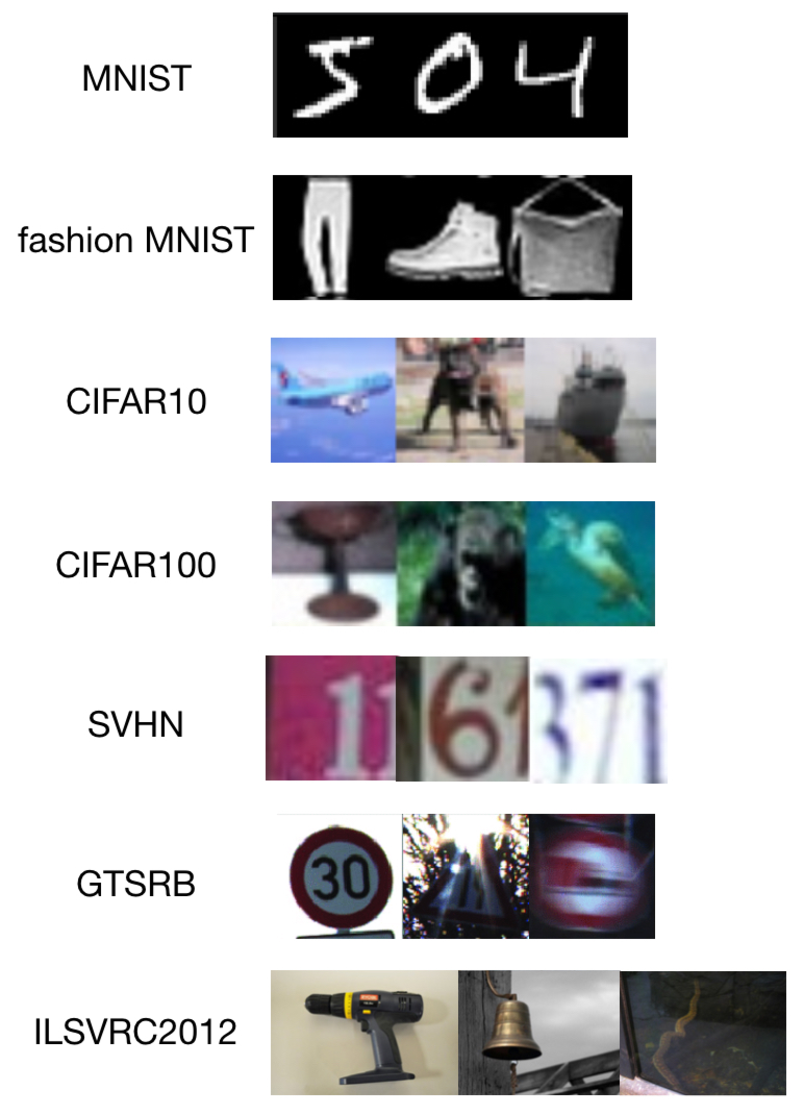
\includegraphics[width=8.0cm]{figures/typical-dataset-samples.pdf}
\end{center}
\caption{
典型的なデータセットのサンプル例.
画像はそれぞれのデータセットから引用.
}
\label{fig:typical-dataset-samples}
\end{figure}
%
